\graphicspath{{chapters/images/06}}

\chapter{17/03/2022}

\section{RDP classifier}

\subsection{Leave-one-out cross validation}

\textbf{How to measure the goodness of a classifier?}
Take out of one data point from the training set,  Apply the classifier on the left-out point (without using it in the training set) Check the accuracy of the prediction
• Repeat the procedure for each training data point. 
\\
RDP classification accuracy evaluated with the leave-one-out
cross validation on the training set of hundreds thousands of 16S
references. The differences are looked over the taxonomic levels, with longer sequences it is possible to evaluate better the taxonomic appartenenza. Obviously, the precision diminishes when checking smaller taxonomic ... %don't remember the name
\\
In real applications, sequencing errors can make this plot worse. 
\\
The classification of bacterias is actually better with variable regions. 

\section{Intro into diversity analysis}

How can I compare two environments for example?
\\
\alpha and \beta diversity: 

\begin{itemize}
	\item \beta -diversity represents how similar two microbial communities are, it's a between sample diversity. The easiest way to estimate it is to take the inverse of the number of shared species.  
	\item \alpha -diversity:  diversity is a measure of how comple a microbial community is, it is considerable as the within sample diversity. The simplest \alpha diversity measureis the species richness. OTU with non-0 abundance. High alpha diversity are associated with macrocommunities robust to external perturbations. 
\end{itemize}

\subsection{Unifrac}
Estimator of \beta -diversity, where distance represents the fraction of the total branch length that is unique to any particular environment.

\begin{figure}[h]
\caption{different colours represent different communities. The horizontal length represents the length of the evolutionary clock. Which OTUs are shared. Percentage between 0 and 1 (?)} %TODO
\centering
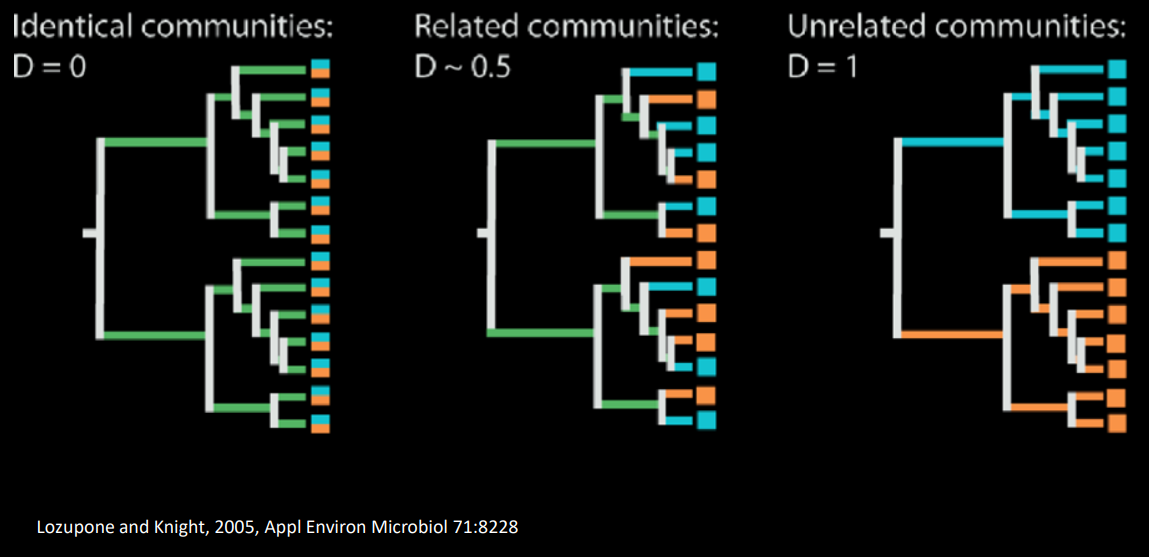
\includegraphics[width=0.6\textwidth]{UniFrac}
\end{figure}

\\

a Distance matrix can be constructed, with the distances between I don't know. 
Through a PCoA it is generated a graph in 2-dimensions. 

\begin{figure}[h]
\caption{}
\centering
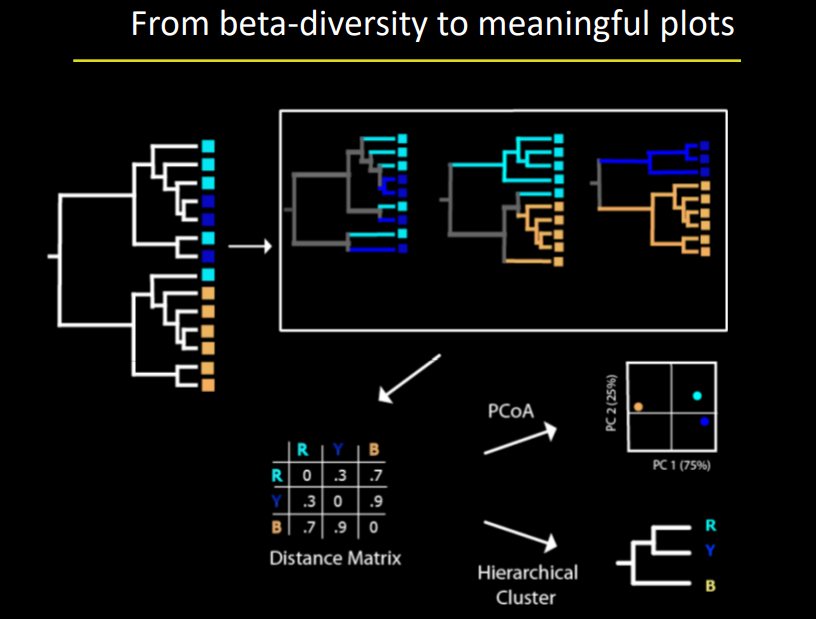
\includegraphics[width=0.6\textwidth]{pCoA}
\end{figure}

A hierarchical cluster represents the relation between samples. The graphs are not considering the abundances of OTUs. The weighted UniFrac estimates the abundance of the OTUs. 
\cite{lozuponeQuantitativeQualitativeBeta2007}

\subsection{Principal coordinate analysis (PCoA)}
multi-dimensional scaling. The ideal concept would be to represent samples in a two or three dimensional space. Principal Coordinate Analysis, Any similarity function can be used (Euclidean distance, UniFrac, BrayCurtis distance). While interpreting clustering results it is important to not overestimate the clusters. 

\section{Experiment of Dassi and collegues}
%TODO



The digestive tract microbiome is generally composed ...
\begin{figure}[h]
\caption{}
\centering
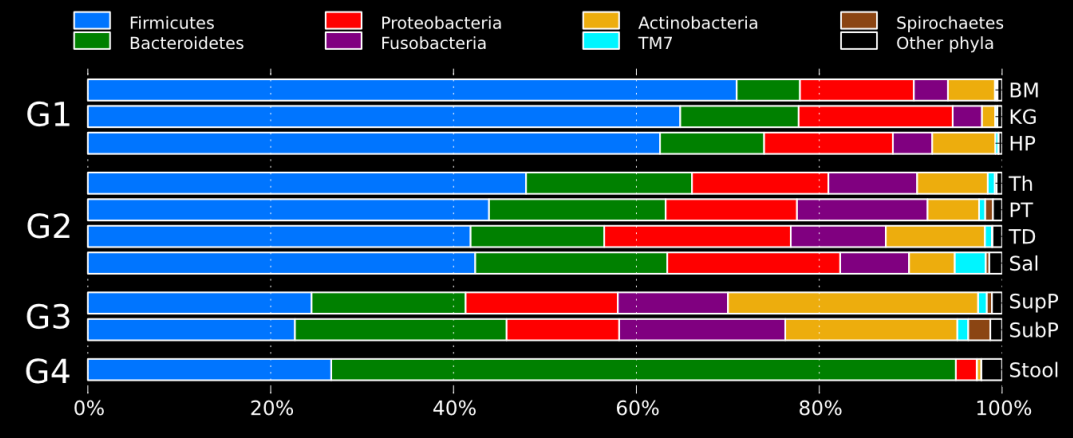
\includegraphics[width=0.6\textwidth]{gut microbes}
\end{figure}


\textbf{Core OTUs}: the OTUs in common are different depending on the variable region considered
\\
Total richness analysis: The overall richness of human saliva continues to increase when  considering more subjects. 


\chapter{Shotgun Metagenomics}
having a microbiome sample, it is extracted the DNA. It is done the sequencing of some variable regions, generating a FastQ file. The data obtained with different samples are with a sixze of about Tbs. It is done the quality control of the reads, and the removal of the contaminant DNA. The analysis is then done. Assembly-based profiling, read-based taxonomic profiling, read-based metabolic profiling. Everything is done wiht reference genomes. 
Metadata information ...

The results have to be tested with independent cohorts. 

\section{Advantages 16S sequencing}
it's less expensive.  avoids non-bacterial contaminations, the resulting dataset is reasonable in size and complecity.

The problems: it's not genome-wide, has limited taxonomic resolution (differences usually don't allow to recognize different bacteria). Cannot see viruses anad eukaryotes. Several biases, ...
Shotgun sequencing instead permits to see the entire genome. High taxonomic resolution. It is also better for cross-study comparisons, can also suvay all domains simultaneously. It is more  expensive, altough the sequencing becomes cheaper and cheaper. It is difficult to remove DNA contamination, can miss low abundance bacteria, the resulting dataset is diffult to process. 

